W ramach projektu postanowiono poddać symulacji wytrzymałościowej również koła zębate.
    Z racji relatywnie dużych przełożeń poddano analizie wyłącznie parę kół zębatych wprowadzającą moment z bębna.
    Najbardziej obciążonymi rejonami w tym przypadku są współpracujące zęby.
    Oprócz tego występuje tutaj płaski stan naprężeń, co pozwala na uproszczenie symulacji do przypadku 2D (geometria na rysunku \ref{fig::geometria_plus_BC_przekladnia}). 
    Do obliczeń za materiał przyjęto stal konstrukcyjną.
    W symulacji zastosowano następujące warunki brzegowe:
    
    \begin{itemize}
    	\item Do wewnętrznej krawędzi większego koła zębatego przyłożono moment obrotowy o wartości 60 Nm (Obciążenie przenoszone z bębna). Oprócz tego nadano jej więz przemieszczeniowy, blokujący ruch w kierunku promieniowym.
    	\item Na powierzchniach styku zębów ustawiono warunek kontaktu z tarciem.
    	\item Wewnętrznej krawędzi mniejszego koła zębatego nadano więz przemieszczeniowy blokujący ruch w kierunku promieniowym oraz wymuszujący zadany obrót. Dzięki czemu uzyskano wyniki dla całego zakresu współpracy kół, dając pewność że znaleziono maksymalne naprężenia pojawiające się w obu elemenetach. 
    \end{itemize}
    

    \begin{figure}[th]
    	\centering
    	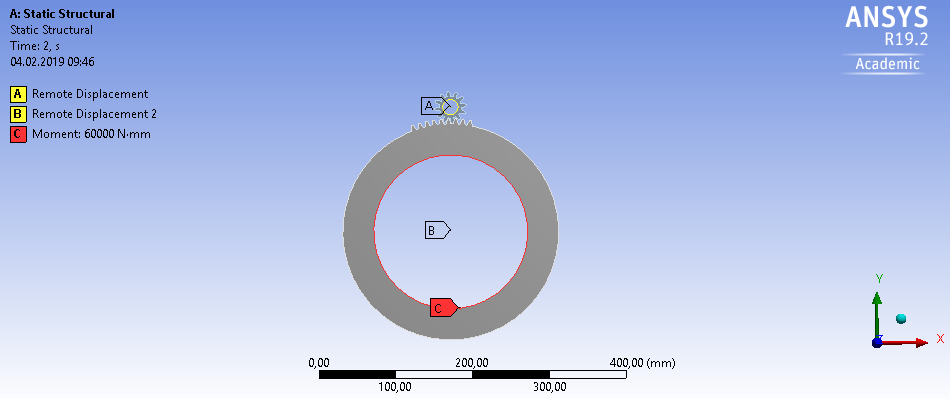
\includegraphics[width=0.9\linewidth]{Obliczenia/geometria_plus_BC_przekladnia}
    	\caption{Uproszczona geometria(usunięto zęby znajdujące się daleko od obszaru współpracy) użyta do wykonania symulacji.} 
    	\label{fig::geometria_plus_BC_przekladnia}
    \end{figure}

Znaczna część geometrii została podzielona siatką o dość dużych elementach, ponieważ nie przenoszą one znacznych obciążeń.
Jedynymi miejscami gdzie wykonano siatkę o dużej rozdzielczości są współpracujące zęby.
Dyskretyzacji dokonano z następującymi parametrami:
\begin{itemize}
	\item Na krawędziach styku nadano podział elementami o boku długości 0,027 mm. 
	Dodatkowo od obu krawędzi w głąb powierzchnii użyto funkcji inflation z pierwszą warstwą o grubości 0,01mm.
	Pozwoliło to uzyskać wysoką rozdzielczość na powierzchnii kontaktu obu ciał oraz zaraz pod nią, gdzie pojawiają się największe gradienty naprężeń.
	\item Reszta powierzchnii obu zębów wraz z ich niewielkim otoczeniem jest podzielona na elementy o boku 0,2mm.
	
\end{itemize}

\begin{figure}[bh]
	\centering
	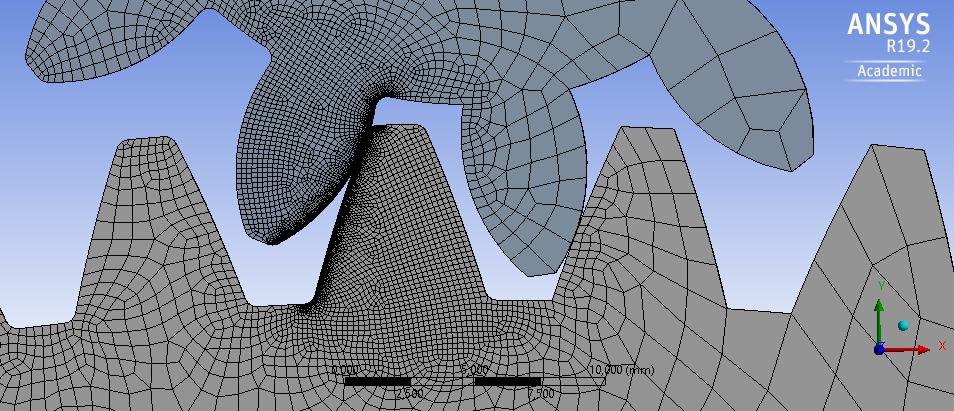
\includegraphics[width=0.9\linewidth]{Obliczenia/siatka_przekladnia}
	\caption{Siatka elementów skończonych użyta w opisywanej symulacji.} 
	\label{fig::mesh_przekladnia}
\end{figure}

Wyniki obliczeń przedstawiono na rysunku \ref{fig::stress_von_mises_przekladnia} w postaci naprężeń zredukowanych.
Jak widać naprężenia na znaczącym poziomie pojawiają tylko w pobliżu strefy kontaktu.
Z racji na ich wartość (259,97 MPa) zdecydowano, że koła zębate muszą być wykonane ze stali konstrukcyjnej C55 ulepszanej cieplnie do Re=540 MPa.
Zapewni to doraźny współczynnik bezpieczeństwa n=2,07.

\begin{figure}[th]
	\centering
	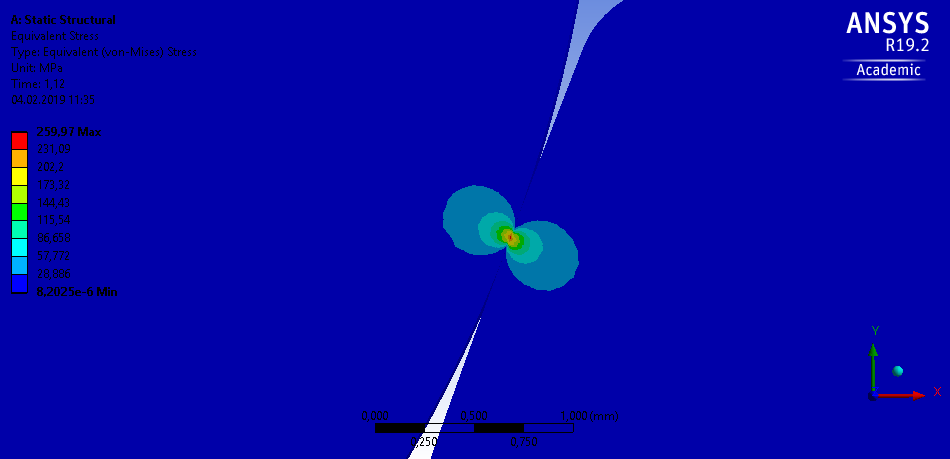
\includegraphics[width=0.9\linewidth]{Obliczenia/von_mises_stress_przekladnia}
	\caption{Naprężenia zredukowane (von Mises) w pobliżu rejonu kontaktu, dla ułożenia kół w którym występują najwyższe naprężenia zredukowane} 
	\label{fig::stress_von_mises_przekladnia}
\end{figure}

\begin{figure}[t]
	\centering
	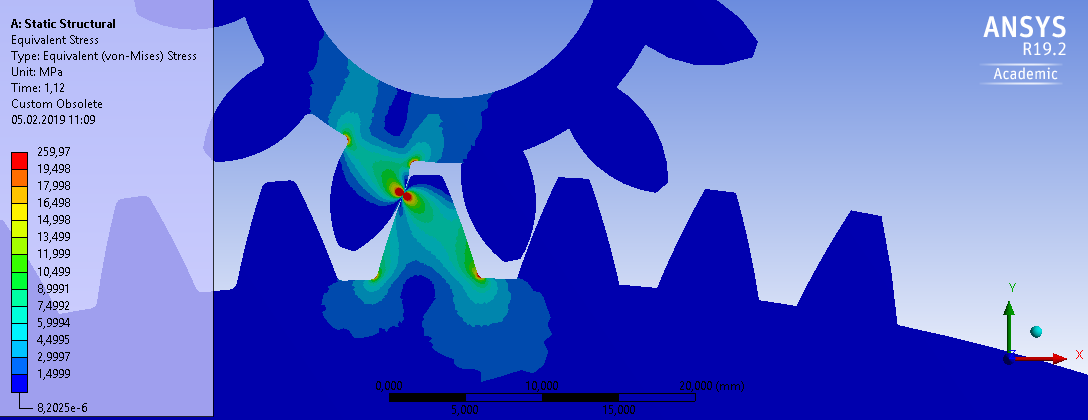
\includegraphics[width=0.9\linewidth]{Obliczenia/von_mises_stress_przeszkalowany_przekladnia}
	\caption{Naprężenia zredukowane (von Mises) w obu współpracujących zębach przy zmienionej skali (ułożenie kół jak poprzednio)} 
	\label{fig::stress_von_mises_przeskalowany_przekladnia}
\end{figure}

W następnym kroku postanowiono dodatkowo sprawdzić elementy pod kątem zmęczeniowym.
W tym celu najpierw zakładana jest twardość materiału:
\begin{equation}
HB=320
\end{equation} 
To z kolei pozwala określić krytyczne naprężenia stykowe oraz zmęczeniowy współczynnik bezpieczeństwa:
\begin{equation}
\sigma_H = 2HB+70 [MPa]= 710MPa
\end{equation}
\begin{equation}
\ N_H=\frac{710 MPa}{259,97 MPa}=2,73
\end{equation} 

Naprężenia otrzymane w symulacji są niższe.
Zatem zgodnie z teorią Woehlera analizowana para kół zębatych nie osiągnie kresu wytrzymałości zmęczeniowej.

Oprócz najbardziej znaczących naprężeń stykowych, zęby są również zginane.
Co więcej moment zginający nie jest stały ze względu na przemieszczanie się punktu przyporu.
Do poniższych obliczeń wybrano moment w którym naprężenia od zginania są maksymalne.
Na rysunku \ref{fig::stress_von_mises_przeskalowany_przekladnia} widać, że maksymalne naprężenia występujące u podstawy zęba wynoszą:

\begin{equation}
\sigma_zg =26MPa
\end{equation}

Rozważany przypadek zginania można uznać za odzerowy tętniący, stąd granica zmęczenia i współczynnik bezpieczeństwa:

\begin{equation}
\ Z_{gj} = 490MPa
\end{equation}
\begin{equation}
\ N_{gj}=\frac{490 MPa}{26 MPa}=18,85
\end{equation} 

Obliczony współczynik pokazuje, że pod wględem zmęczenia związanego ze zginaniem u podstawy zęba, nie istnieje tutaj żadne zagrożenie.

Następnie postanowiono sprawdzić zakres kontaktu. 
Zrobiono to poprzez analizę poślizgu punktów znajdujących się na stykających się powierzchniach (Rysunek \ref{fig::zakres_kontaktu}). 
Pokazuje on, że w części strefy kontaktu występują dodatnie naprężenia styczne (ujemny poślizg) w drugiej zaś przeciwnie.
W przypadku zakresu dodatniego maksymalna wartość to $\tau_+$=35,7 MPa, zaś dla ujemnego $\tau_-$=-33,24 MPa.
Oprócz tego występuje punkt gdzie nie występuje poślizg, zatem nie będzie tam również naprężeń stycznych.
Ponadto układ naprężeń stycznych będzie skierowany na zewnątrz punktu bez poślizgu.
Poza wymienionymi informacjami, analiza ta pokazując zakres kontaktu pozwala na określenie możliwego zakresu podcięcia technologicznego symulowanych zębów.


\begin{figure}[th]
	\centering
	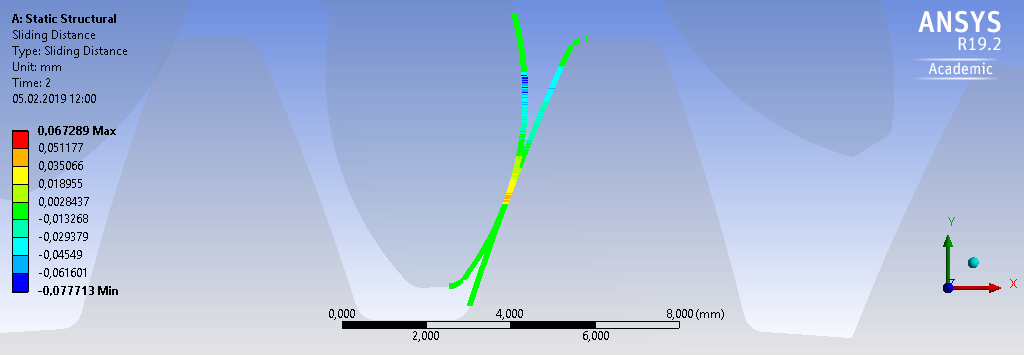
\includegraphics[width=0.9\linewidth]{Obliczenia/zakres_kontaktu}
	\caption{Poślizg na stykających się powierzchniach kół zębatych} 
	\label{fig::zakres_kontaktu}
\end{figure}

Na koniec przeanalizowano siłę reakcji między zębami na kierunku obwodowym.
Na początku przebiegu widoczny jest liniowy wzrost związany ze stopniowym przykładniem obciążenia przez program.
W dalszej części widać, że siła jest stała.
Potwierdza to dobrą jakość odwzorania ewolwenty i spełnia wymagane we wcześniej fazie projektu stałe przełożenie.

\begin{figure}[th]
	\centering
	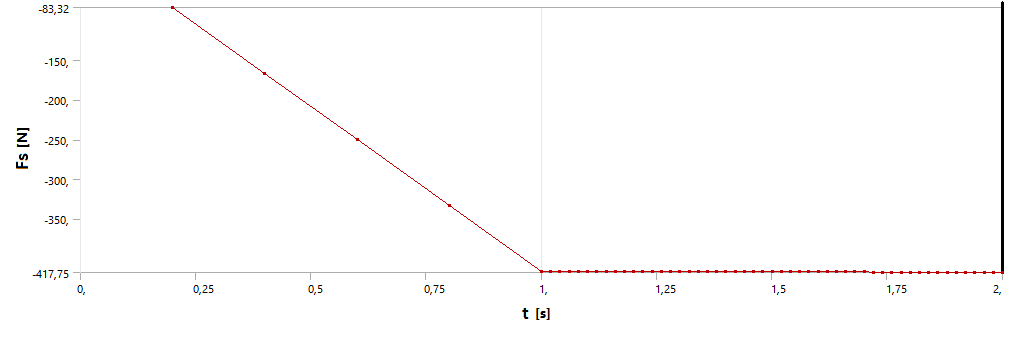
\includegraphics[width=0.9\linewidth]{Obliczenia/sila_reakcji_obwodowa_w_zebie}
	\caption{Siła reakcji między zębami na kierunku obwodowym} 
	\label{fig::sila_obwodowa}
\end{figure}

